%Chapter 3

\renewcommand{\thechapter}{3}

\chapter{Methodology}

\section{Introduction}
As previously stated, our team has attempted to answer our research questions by developing a mathematical model 
and evaluating its accuracy with a experimental model.  Our research questions are:

\begin{enumerate}
    \item[(1)]
    How can the dynamic charging of EVs be successfully implemented into a roadway?  
    \item[(2)]
    Would dynamic charging be able to provide enough power to a vehicle to make a difference in its overall range capability? 
    \item[(3)]
    Is dynamic charging a safe and reliable means of transmitting power to a vehicle in motion on the roadway, and would it affect a vehicle’s performance in other ways?   
    \item[(4)]
    Would a traditional roadway be able to accommodate dynamic charging, or would more nontraditional infrastructure need to be created?
\end{enumerate}

\section{Hypothesis}
By testing different values for the variables listed below, we can develop a recommendation to optimize the power 
output efficiency of a prototype of a dynamic wireless power transfer (DWPT) system for an electric vehicle (EV).
Variables:
\begin{itemize}
    \item Voltage of source [V]
    \item Wire gauge of transmitting coil []
    \item Number of turns in transmitting coil []
    \item Radius of transmitting coil [m]
    \item Wire gauge of receiving coil []
    \item Number of turns in receiving coil []
    \item Radius of receiving coil [m]
    \item Height of the receiving coil above the transmitting coil [m]
    \item Distance between closest edges of coils in road [m]
    \item Velocity of car [m/s]
    \item Material that encloses the transmitting and receiving coil []
    \item Alignment with coil []
\end{itemize}

Through our research we were able to develop a model that incorporates all of the variables except material and 
alignment of coil, although further research could be done to incorporate these variables.

\section{Simulations}
Our simulation is coded in MATLAB R2020a using basic characteristics of MATLAB and the Parallel Computing Toolbox 
in order to run simulations at a faster speed when possible. By starting with the verified and validated Biot 
Savart Magnetic Toolbox for MATLAB, a toolbox used for numerically calculating the magnetic field of filaments 
in a 3D field, a full DWPT simulation was able to be developed \cite{lqueval_lquevalbsmag_2020}. The simulations use two modified 
functions from the toolbox, BSmag\_add\_filament.m and BSmag\_get\_B.m and functions get\_field.m and get\_flux.m 
developed with some help from the toolbox, as well as a main.m which is responsible for running a batch 
(more than one) of scenarios. Each function is explained in detail below.

\subsection{General Approach}
The purpose of the simulations is to provide an estimate of the total charge a given configuration can provide 
to a car battery over a given distance, as well as the relative cost of that configuration to the persons building it.  
We don’t consider the costs of car owners to be a barrier to adoption, because the cost is negligible for each owner 
in comparison to the cost of the infrastructure. As previously explained in Section \ref{sec: s2.3}, the flux through 
a coil needs to be calculated in order to determine the induced current in the receiving coil. The first component 
of flux is magnetic field, so the field must be calculated for a 3D matrix of points surrounding the transmitting. 
This is the main purpose of the Biot Savart Toolbox. Once the field is plotted, the total flow through the imaginary 
“surface” created by the receiving coil must be calculated by adding up the field at each point of the receiving coil 
over its area. Finally, the induced emf can be calculated by numerically integrating the flux over time and the 
current can be determined using Ohm’s Law and the calculated resistance of the receiving coil. Since current is a 
flow of charge, the charge to the battery can be obtained by integrating the current over time.

While the concepts behind the simulation are simple, the computations quickly become unwieldy, 
which required much optimization of the simulation in order to prevent unnecessary repeated computations. 
This led to a segmented design where the configuration of the infrastructure, or the environment, is only 
calculated once for each unique configuration although there are many car configurations that can be “driven” 
through each. We made assumptions that edge effects are negligible compared to the effects of the nearby coils 
and ran the simulation for 1600 m (approximately 1 mile) for all scenarios. Both the numerical plotting of the 
magnetic field and the numerical integration of the flux through the car’s coil are hefty calculations which is 
why the Parallel Computing Toolbox is necessary to run a large batch of simulations. With 10 variables being 
considered, even trying 2 values for each value is not an insignificant task (210 = 1024). This required much 
discretion in terms of deciding which variables to spend time testing more rigorously. 

\subsection{BSmag\_add\_filament.m}
The function prototype is:
\begin{center}
function [BSmag] = BSmag\_add\_filament(BSmag, Gamma, I, dGamma)
\end{center}
The purpose of this function is to add a filament, 
in our case a coil, to the 3D space. It takes the following 
inputs and outputs to accomplish this shown in Table \ref{t1} and Table \ref{t2}:

\begin{table}[H]
    \caption[BSmag\_add\_filament.m Inputs]{BSmag\_add\_filament.m Inputs}
    \begin{center}
    \begin{tabular}{| p{0.2\textwidth} | p{0.1\textwidth} | p{0.6\textwidth} |}
    \hline
    Input & Units & Purpose \\
    \hline \hline
    BSmag & & The BSmag data structure that is at first empty but each time a filament is added, it holds the new number of filaments as well as the characteristics of each filament (Gamma, I, dGamma). \\
    Gamma & [m, m, m] & The filament point coordinates, in our case we translate a linearly spaced vector in radians to x, y, and z coordinates. \\
    I & [A] & The current through the coil, where the sign indicates the direction. \\
    dGamma & [m] & The filament max discretization step. \\
    \hline
    \end{tabular}
    \end{center}
    \label{t1}
\end{table}

\begin{table}[H]
    \caption[BSmag\_add\_filament.m Outputs]{BSmag\_add\_filament.m Outputs}
    \begin{center}
    \begin{tabular}{| p{0.2\textwidth} | p{0.1\textwidth} | p{0.6\textwidth} |}
    \hline
    Output & Units & Purpose \\
    \hline \hline
    BSmag & & The BSmag data structure updated to include the nth filament. This can be passed back into the function any number of times to add more filaments. \\
    \hline
    \end{tabular}
    \end{center}
    \label{t2}
\end{table}

Prior to calling this function it’s important to set the number of total filaments in the BSmag object to 0, 
so that it starts fresh for each scenario. In our simulations, we assume that the direction of current is 
alternating so each time a coil is added the sign of the current is reversed. As stated previously, 
this function was taken from the Biot Savart Toolbox, but unnecessary information was removed to improve 
performance \cite{lqueval_lquevalbsmag_2020}.

\subsection{BSmag\_get\_B.m}
The function prototype is:
\begin{center}
    function [X,Y,Z,BZ] = BSmag\_get\_B(BSmag, X, Y, Z, muRel)
\end{center}
The purpose of this function is to calculate the magnetic field 
for all points in the specified 3D space made up of X, Y, Z. It takes the following inputs and outputs to accomplish 
this as shown in Table \ref{t3} and Table \ref{t4}:

\begin{table}[H]
    \caption[BSmag\_get\_B.m Inputs]{BSmag\_get\_B.m Inputs}
    \begin{center}
    \begin{tabular}{| p{0.2\textwidth} | p{0.1\textwidth} | p{0.6\textwidth} |}
    \hline
    Input & Units & Purpose \\
    \hline \hline
    BSmag & & The BSmag data structure that includes information about the filaments. \\
    X & & Field points x-coordinate vector or matrix. \\
    Y & & Field points y-coordinate vector or matrix. \\
    Z & & Field points z-coordinate vector or matrix. \\
    muRel & & The relative permeability of the material. \\
    \hline
    \end{tabular}
    \end{center}
    \label{t3}
\end{table}

\begin{table}[H]
    \caption[BSmag\_get\_B.m Outputs]{BSmag\_get\_B.m Outputs}
    \begin{center}
    \begin{tabular}{| p{0.2\textwidth} | p{0.1\textwidth} | p{0.6\textwidth} |}
    \hline
    Output & Units & Purpose \\
    \hline \hline
    X & & Field points x-coordinate vector or matrix. \\
    Y & & Field points y-coordinate vector or matrix. \\
    Z & & Field points z-coordinate vector or matrix. \\
    BZ & [T] & The z-component of the magnetic field. \\
    \hline
    \end{tabular}
    \end{center}
    \label{t4}
\end{table}

The function takes a term muRel which we assume to be 1 in our simulations. The term was included in order to 
make it easier for future research to incorporate it by estimating the composite permeability of the material 
between the transmitting coils and the receiving coils. This could include asphalt or concrete that may obscure 
the coil in the road, air, and any components on the vehicle that may obscure the coils.  By setting muRel = 1, 
we assume vacuum permeability which is a limitation of our experiments. It’s a source of over overestimation 
of the results because the space between the coils is not actually as permeable as a vacuum, but since the space 
is made up of mostly air it is a fair assumption. As stated previously, this function was taken from the Biot 
Savart Toolbox, but unnecessary information was removed to improve performance \cite{lqueval_lquevalbsmag_2020}.  
This is why the function used in our simulations only returns the z-component of the field. We assume that the coils 
are aligned perfectly parallel to one another and the road, so the only component of the field that has an effect on 
the flux through the receiving coil is the perpendicular component, or the z-component. In reality they are not 
perfectly parallel and edge affects can have effects, so this is a limitation of our simulation and a source of error. 

\subsection{get\_field.m}
The function prototype is:
\begin{center}
    function data = get\_field(V, wireGauge, turns, radius, wireGauge\_car, turns\_car, radius\_car, height, original\_spacing, velocity, scenarioID, outputFolder)
\end{center}
The purpose of this function is to calculate the magnetic 
field and cost of the provided configuration and pass relevant information to get\_flux.m for each configuration 
of the car. It then returns a matrix of all of the inputs for each unique scenario, the cost, and the total charge 
calculated by get\_flux.m. It takes the following inputs and outputs to accomplish this as shown in 
Table \ref{t5} and Table \ref{t6}:

\begin{table}[H]
    \caption[get\_field.m Inputs]{get\_field.m Inputs}
    \begin{center}
    \begin{tabular}{| p{0.2\textwidth} | p{0.1\textwidth} | p{0.6\textwidth} |}
    \hline
    Input & Units & Purpose \\
    \hline \hline
    V & [V] & The voltage of the source. \\
    wireGauge & [] & The wire gauge of the transmitting coils. \\
    turns & [] & The number of turns of the transmitting coils. \\
    radius & [m] & The radius of the transmitting coils. \\
    wireGauge\_car & [] & The wire gauge of the receiving coil. \\
    turns\_car & [] & The number of turns of the receiving coil. \\
    radius\_car & [m] & The radius of the receiving coil. \\
    height & [m] & The vertical distance between the transmitting and receiving coils. \\
    original\_spacing & [m] & The distance between the closest parts of the transmitting coils. \\
    velocity & [m/s] & The velocity of the car. \\
    scenarioID & [] & The identifier for this unique 3D configuration of the environment. \\
    outputFolder & & The folder where any figures and data will be written. \\
    \hline
    \end{tabular}
    \end{center}
    \label{t5}
\end{table}

\begin{table}[H]
    \caption[get\_field.m Outputs]{get\_field.m Outputs}
    \begin{center}
    \begin{tabular}{| p{0.2\textwidth} | p{0.1\textwidth} | p{0.6\textwidth} |}
    \hline
    Output & Units & Purpose \\
    \hline \hline
    data & & The matrix that contains the unique inputs and outputs (total charge and cost) for each unique configuration of the receiving coil for the current configuration of the environment. \\
    \hline
    \end{tabular}
    \end{center}
    \label{t6}
\end{table}

The function also has a list of constants which are important for subsequent calculations shown in Table \ref{t7}.

\begin{table}[H]
    \caption[FORMULA Constants]{FORMULA Constants}
    \begin{center}
    \begin{tabular}{| p{0.2\textwidth} | p{0.15\textwidth} | p{.1\textwidth} | p{0.45\textwidth} |}
    \hline
    Input & Value & Units & Purpose \\
    \hline \hline
    increment & .1 & [m] & The resolution or the distance between the points in the 3D meshgrid. This needs to be one order of magnitude less than any inputs in order for best performance. \\
    muRel & 1 & [] & The relative permeability of the material. \\
    rho & .0171E-6 & [ohm-m] & The resistivity of copper. \\
    density & & [g/m3] & The density of copper. \\
    wireGauges & array & [] & An array of wire gauges needed all configurations. \\
    WireDiameters & array & [m] & n array of corresponding diameters to the wire gauge array. \\
    maxDistance & 1600 & [m] & The total distance traveled by the simulated car. In all simulations we used 1600 m or approximately 1 mile to determine the predicted charge per mile. \\
    dGamma & 1E9 & [m] & The filament max discretization step. \\
    filamentStep & 10 $\cdot$ radius & [1/m] & The number of points in each turn of the transmitting coils. Increase for better performance. \\
    tightness & 10000 & [1/m] & The tightness with which the coils are wrapped. Increasing tightness will make the coils wrapped more tightly, but we use a sufficiently large number so that it is as if the coils are wrapped perfectly tightly. \\
    \hline
    \end{tabular}
    \end{center}
    \label{t7}
\end{table}

This function does a series of numerical calculations to calculate the field in the specified 3D space. 
First, it determines coil characteristics from the wire gauges, which also allows the current to be 
calculated using V, resistance, and Ohm’s law. The cost is then calculated using the power (P = IV) 
and weight of wire. The cost also takes into account the cost of the copper wire and the cost of the 
solar panels that would be needed to power the design. In the next section, eight coils are placed on the 
3D space with alternating currents. In the next step the desired 3D matrix is plotted using linearly spaced 
vectors and then the field is calculated by calling BSmag\_get\_B. Next, the scenarios for the desired car 
configurations are determined and get\_flux.m is called for each of them. Finally, the data matrix returns 
the desired information for all of the car configurations for the current configuration of the environment.

\subsection{get\_flux.m}
The function prototype is:
\begin{center}
function totalCharge = get\_flux(turns, d\_car, turns\_car, radius\_car, height, spacing, velocity, rho, scenarioID, BZ, X\_M, Y\_M, increment, meshDistance, heightIndex, numberOfSquaresX, numberOfSquaresY, outputFolder).
\end{center}
The purpose of this function is to calculate the total charge over a specified distance for each configuration 
of the car and returns the value. This function can also be used to plot 3D renderings of the configuration 
and graph charge or current over time, but in the majority of cases this feature is not used because the 
final output is the only information of interest. It takes the following inputs and outputs to accomplish 
this as shown in Table \ref{t8} and Table \ref{t9}. The function also has a list of constants which are 
important for subsequent calculations as shown in Table \ref{t10}.

\begin{table}[H]
    \caption[get\_flux.m Inputs]{get\_flux.m Inputs}
    \begin{center}
    \begin{tabular}{| p{0.25\textwidth} | p{0.1\textwidth} | p{0.55\textwidth} |}
    \hline
    Input & Units & Purpose \\
    \hline \hline
    turns & [] & The number of turns of the transmitting coils. \\
    d\_car & [m] & The diameter of the wire of the receiving coils. \\
    turns\_car & [] & The number of turns of the receiving coil. \\
    radius\_car & [m] & The radius of the receiving coil. \\
    height & [m] & The vertical distance between the transmitting and receiving coils. \\
    spacing & [m] & The distance between the closest parts of the transmitting coils plus the diameter of the transmitting coils. \\
    velocity & [m/s] & The velocity of the car. \\
    rho & [ohm-m] & The resistivity of copper. \\
    scenarioID & [] & The identifier for this unique 3D configuration of the environment and car. \\
    BZ & [T] & The z-component of the magnetic field. \\
    X\_M	& & Field points x-coordinate vector or matrix. \\
    Y\_M	 & & Field points y-coordinate vector or matrix. \\
    increment & [m] & The resolution or the distance between the points in the 3D meshgrid. \\
    meshDistance & [m] & The distance required to calculate the field for all 7 coils. \\
    heightIndex & [] & The index of the node at the desired height in the z-direction. \\
    NumberOfSquaresX & [] & The number of nodes across the x-direction of the meshgrid. \\
    NumberOfSquaresY & [] & The number of nodes across the y-direction of the meshgrid. \\
    outputFolder & & The folder where any figures and data will be written. \\
    \hline
    \end{tabular}
    \end{center}
    \label{t8}
\end{table}

\begin{table}[H]
    \caption[get\_flux.m Outputs]{get\_flux.m Outputs}
    \begin{center}
    \begin{tabular}{| p{0.2\textwidth} | p{0.1\textwidth} | p{0.6\textwidth} |}
    \hline
    Ouput & Units & Purpose \\
    \hline \hline
    totalCharge & [C] & The total charge calculated over the specified distance for the unique configuration. \\
    \hline
    \end{tabular}
    \end{center}
    \label{t9}
\end{table}

\begin{table}[H]
    \caption[FORMULA Constants]{FORMULA Constants}
    \begin{center}
    \begin{tabular}{| p{0.25\textwidth} | p{0.125\textwidth} | p{.075\textwidth} | p{0.45\textwidth} |}
    \hline
    Input & Value & Units & Purpose \\
    \hline \hline
    distanceStep & increment & [m] & The resolution of the distance between each snapshot of the car traveling on the road. Set equal to increment for best results or multiply by some integer multiple for faster (but less accurate) results. \\
    efficiencyOfRectifier & 1 & [] & The efficiency of the rectifier. For our simulations we assume the current is perfectly rectified, although this is an implication and therefore a source of error. \\
    tightness\_car & 10000 & [1/m] & The tightness with which the receiving coils are wrapped. Increasing tightness will make the coils wrapped more tightly, but we use a sufficiently large number so that it is as if the coils are wrapped perfectly tightly. \\
    \hline
    \end{tabular}
    \end{center}
    \label{t10}
\end{table}

This function does a series of calculations to calculate the flux in through the coil as it travels through the 3D 
space. In order to run faster simulations, we use two of the central coils out of the 8 we plotted and then assume 
that through a large space the field is the same, and therefore the flux is the same. This was shown to be a fair 
assumption through tests comparing estimated values to actual values with no significant difference in the outputs. 
For each snapshot in time as the car travels down the road, the flux is calculated by filtering out irrelevant 
field locations and then integrating numerically using the trapz function over the x and y directions. 
Then the flux is copied and pasted to each of the corresponding locations in the array that represents the actual 
distance the car travels.  Using the flux array and corresponding time array, we are able to obtain the total 
charge accumulated in the battery over the desired distance, using numerical versions of the equations:
\begin{equation}
    \mathcal{E} = -N \frac{d\Phi}{dt}
\end{equation}
Where N is the number of turns in the receiving coil, $\Phi$ is the flux, t is the time, and $\mathcal{E}$ 
is the emf induced in the receiving coil. 
\begin{equation}
    I = \frac{\mathcal{E}}{R}
\end{equation}
Where R is the resistance of the coil in the car, and I is the current of the coil in the car.
\begin{equation}
    Q = \int{I dt}
\end{equation}
Where Q is the total charge stored in the battery. 

\subsection{main.m}
main.m function is responsible for calling get\_field.m for each unique 3D configuration of the variables and 
passing in desired values for the car configurations. This function utilizes the Parallel Computing Toolbox 
so that unique environmental configurations can be computed in parallel if multiple CPUs are needed and available. 
The data is written to a text file delimited by commas so that it can easily be imported into other programs for 
analysis. See Section \ref{sec: s4.1} for the values used for the variables and the results of the simulations.

\subsection{analysis.py}
A simple Python script was written in Python 3 in order to produce graphs that show the outputs of the simulations 
against each variable. This was used to determine which variables had the largest effects on the output and what 
configurations had the largest charge to cost ratio.  We know that with infinite resources it would be possible 
to complete this project, but without some idea of the cost to the government or entity completing the project 
the results wouldn’t be very valuable. 

Within the Python script, libraries pydrive \cite{nabel_pydrive_nodate}, google \cite{noauthor_breaking_nodate}, 
oauth2client \cite{noauthor_what_nodate} are used to import required data files. Data are processed as a data frame in 
the pandas library \cite{jeff_reback_pandas-devpandas_2021}, and matplotlib \cite{hunter_matplotlib_2007} is used 
to graph the outputs. For the first batch of data of smaller size, each entry of output data was iterated and compared 
with each other to analyze the target variable while having other variables being fixed. For the second batch of 
data of larger size, possible entries of each variable were iterated in order to fix required variables and analyzed 
target variables. See Section \ref{sec: s4.1} for detailed analysis and Appendix \ref{sec: appB} for code used in Batch 2.

\section{Experimental Model}
To validate the results of our simulations, we designed an experimental model. The experimental model uses a 
circular path to mimic a straight line. It consists of a wooden platform to place the transmitting coils on, 
a rotating metal shaft with another metal arm attached at the top, and a motor to rotate the shaft. 
We used a pulley system with a gear ratio of 1:9.33 to the motor and rotating shaft to control the speed of 
the rotation. The coils used were 1.75” in diameter. We placed 16 of these coils on the platform in a circular 
path and connected them to a power supply to generate an electromagnetic field over each of the coils. 
On the rotating arm, we attached a small wooden car using a threaded rod. The receiving coil was then 
attached to a wooden car using Velcro. As the arm rotated, the receiving coil would have a current induced 
onto it by interacting with the aforementioned electromagnetic field. We wired the receiving coil to a slip 
ring on the rod that would allow the wires to not be tangled as the rod rotated. The wires from the end of 
the slip ring were then connected to an oscilloscope to measure the resulting current that was induced onto 
the receiving coil. 

\subsection{General Approach}
Our goal with the experimental model is to determine how the simulations translate to a real-world scenario. 
We planned on running the model using different variable combinations to find the optimal real-world application 
of this technology; however, due to the COVID pandemic we had to fall back on our original goals. 
Our current goal is to prove that the technology is feasible by showing that there is an electrical 
output from the receiving coil. The experimental model is a proof of concept of the simulations, 
showing that the technology is feasible and could enable EVs to charge while driving.

\subsection{Construction of the Experimental Model}
\subsubsection{Pulley Subsystem}
 
\begin{figure}
    \begin{center}
    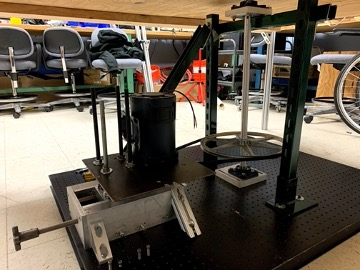
\includegraphics[width=5in]{fig5.jpg}
    \end{center}
    \renewcommand{\baselinestretch}{1}
    \small\normalsize
    \begin{quote}
    \caption[A picture showcasing the pulley subsystem]{A picture showcasing the pulley subsystem} \label{fig: f5}
    \end{quote}
\end{figure}

A 12V DC motor drives the vertical shaft of the rig via a v-belt pulley connection. The motor is mounted to 
a tensioner that maintains the proper belt tension. The tensioner is fixed to the optical breadboard. 
The speed of the motor is controlled by a variable DC power supply. Two ball bearings are used to constrain 
the vertical shaft. The bottom bearing is fixed to a plate that is secured in the optical breadboard. 
The top bearing is fixed to a plate that is supported by a green metal frame that is also connected 
to the optical breadboard. 

\subsubsection{Arm Subsystem}

\begin{figure}
    \begin{center}
    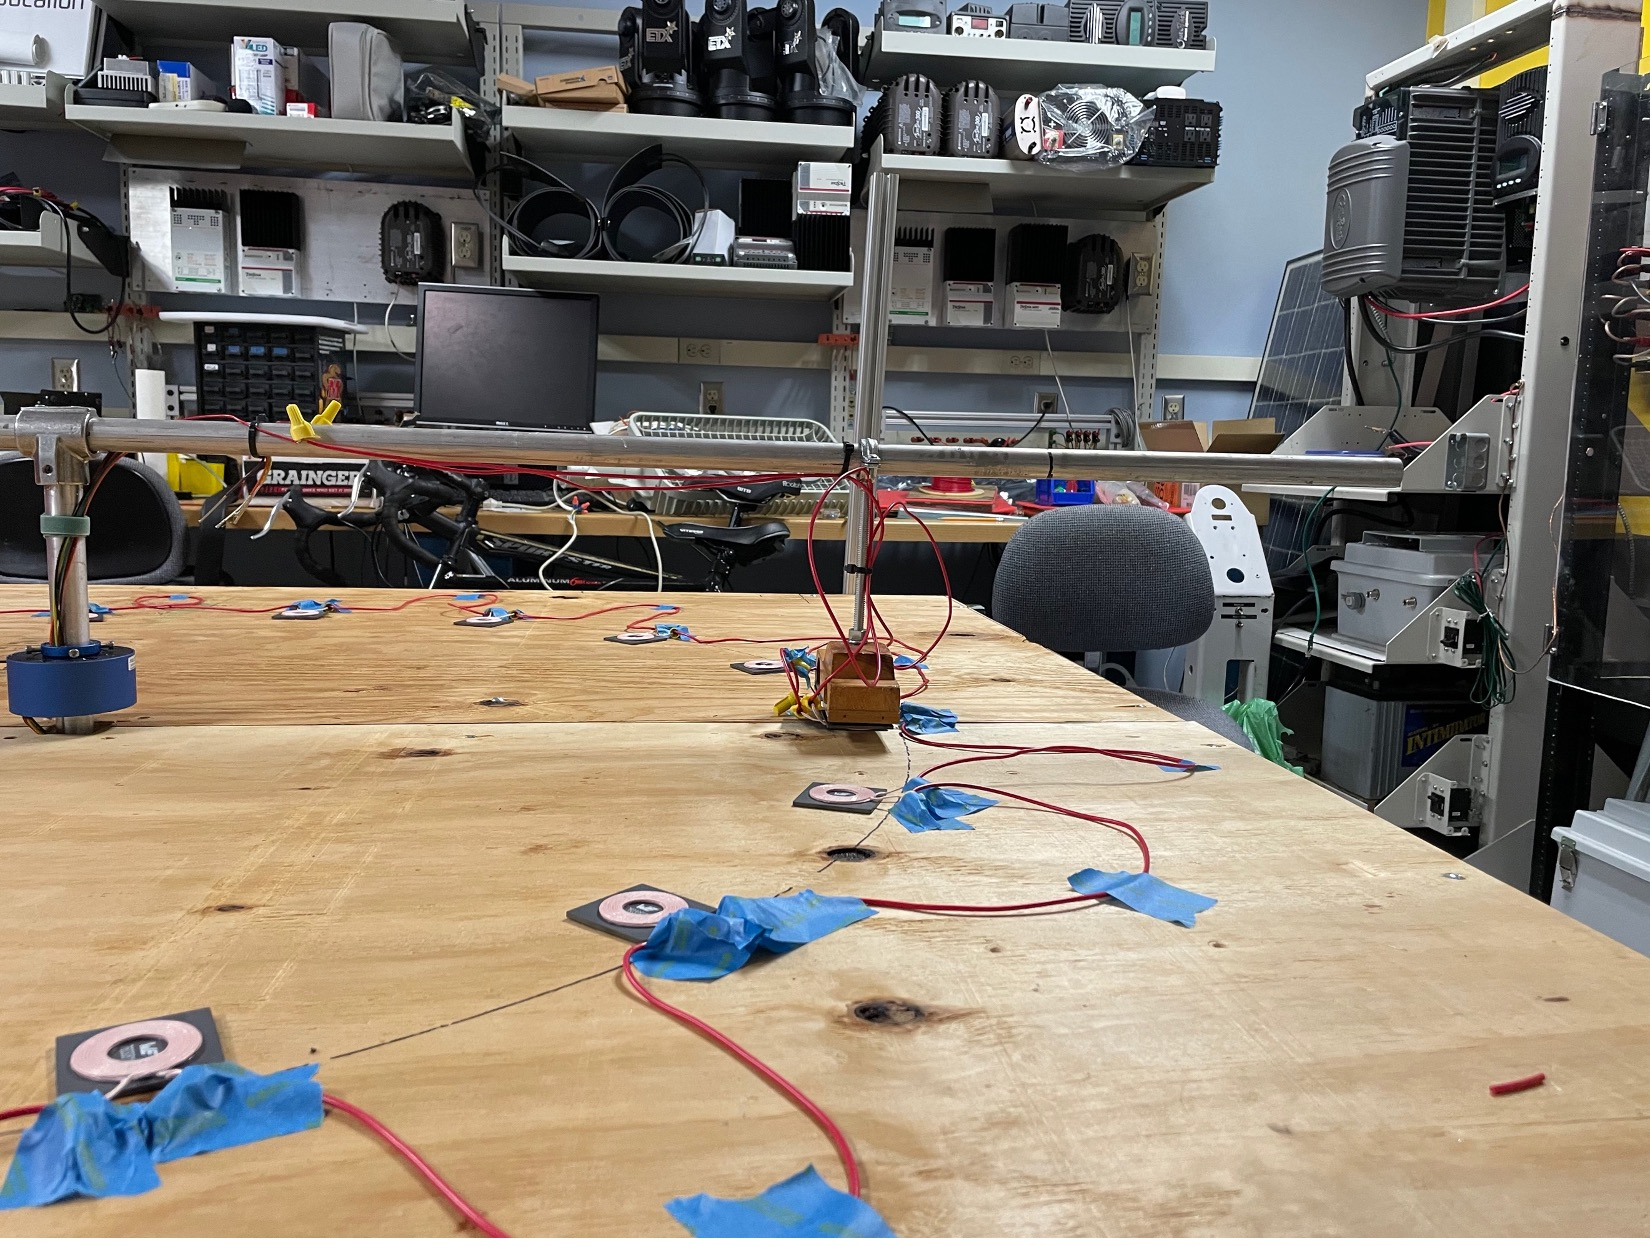
\includegraphics[width=5in]{fig6.jpg}
    \end{center}
    \renewcommand{\baselinestretch}{1}
    \small\normalsize
    \begin{quote}
    \caption[Rotating arm with vehicle attached]{Rotating arm with vehicle attached} \label{fig: f6}
    \end{quote}
\end{figure}

An aluminum T-connector connects the vertical shaft to the arm. This allows the arm to rotate at a 
constant angular velocity corresponding to the stepped down speed of the motor. The “vehicle” is 
mounted to the arm and travels in a circle to simulate DWPT. A slip ring is attached to the vertical 
shaft below the t connector. This prevents the wiring that travels along the arm from getting twisted 
as the rig rotates. 

\subsubsection{Transmitting Coils}

\begin{figure}
    \begin{center}
    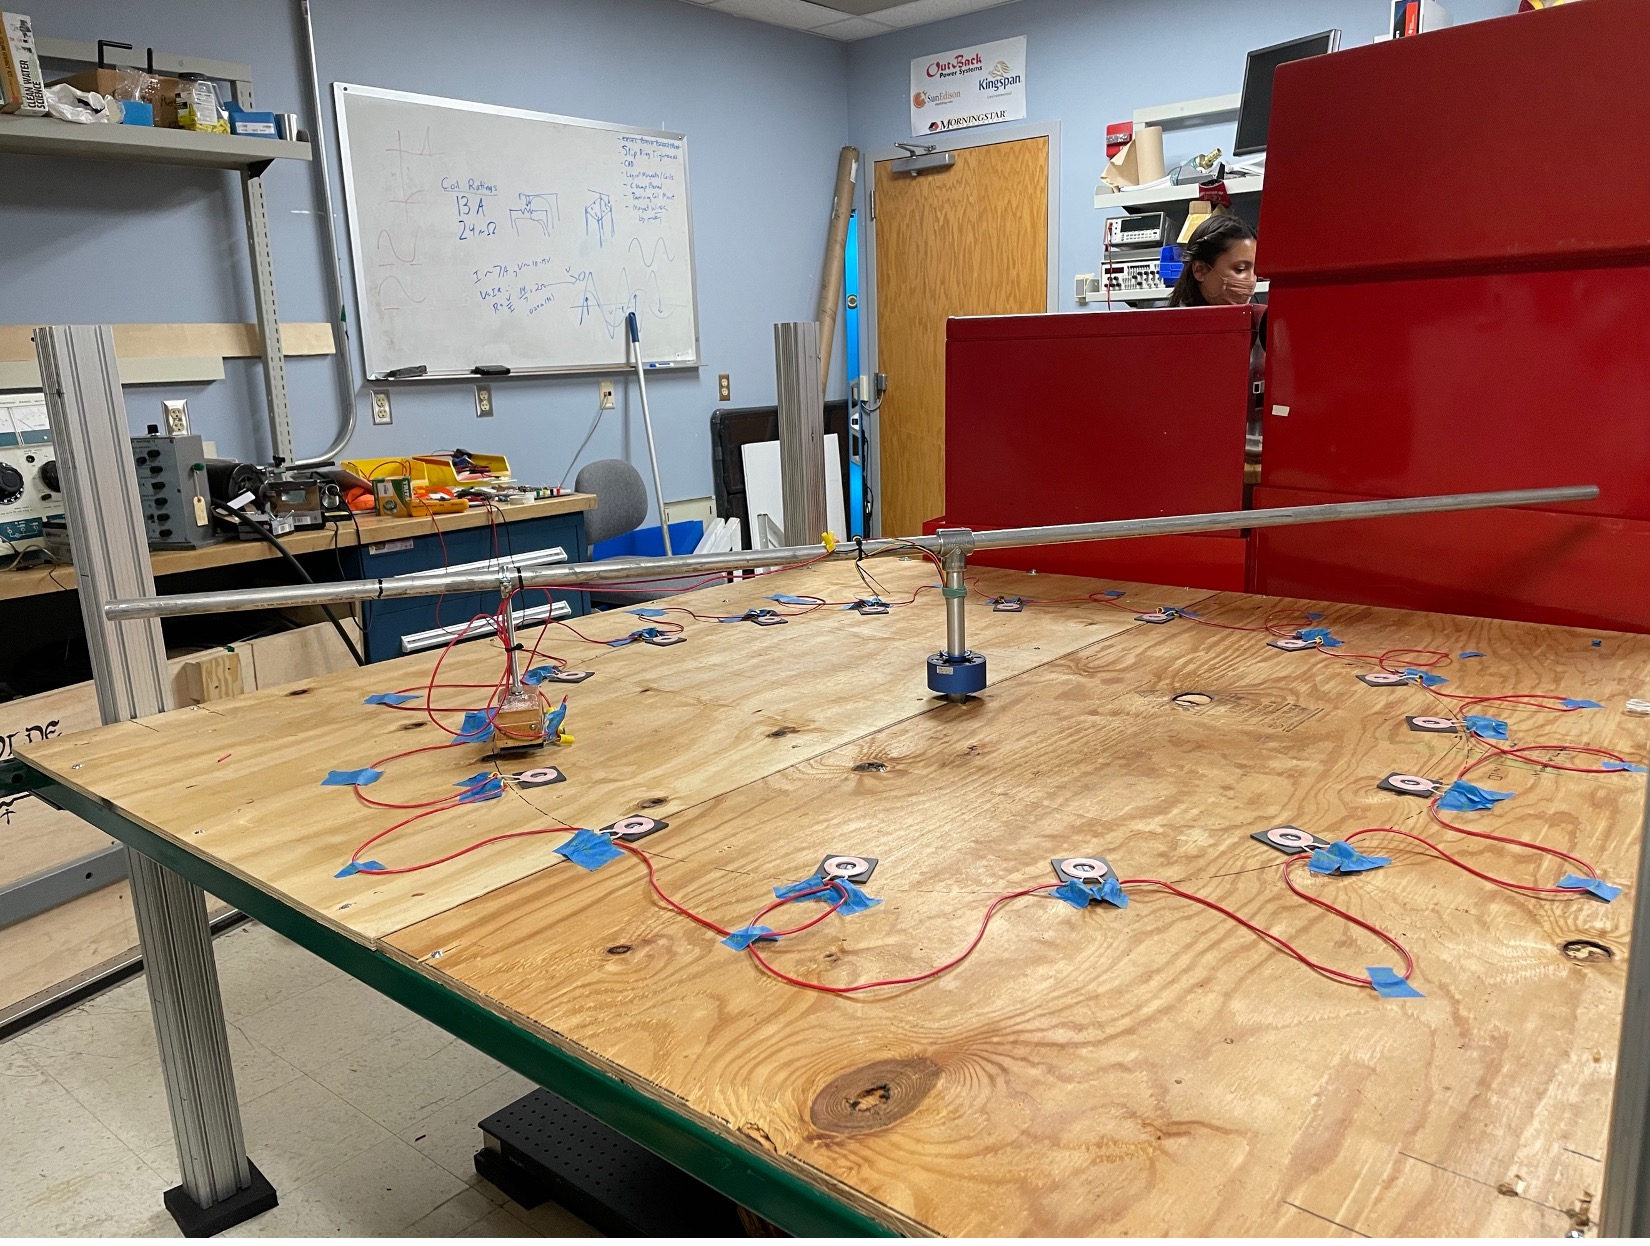
\includegraphics[width=5in]{fig7.jpg}
    \end{center}
    \renewcommand{\baselinestretch}{1}
    \small\normalsize
    \begin{quote}
    \caption[Transmitting coils laid out in a constant diameter]{Transmitting coils laid out in a constant diameter} \label{fig: f7}
    \end{quote}
\end{figure}

16 - 1.75” diameter coils are spaced evenly around a 2 ft diameter circle from the center of the experimental model. 
The coils are connected in series and powered through a variable DC power supply. Wire nuts are used to 
electrically insulate all connections. The total resistance of the coils is 0.3 $\Omega$ and the current 
rating is 11 A. These transmitting coils represent the coils that would be embedded in the road and transmit 
power to the passing electric vehicle.

\subsubsection{Receiving Coils}
 
\begin{figure}
    \begin{center}
    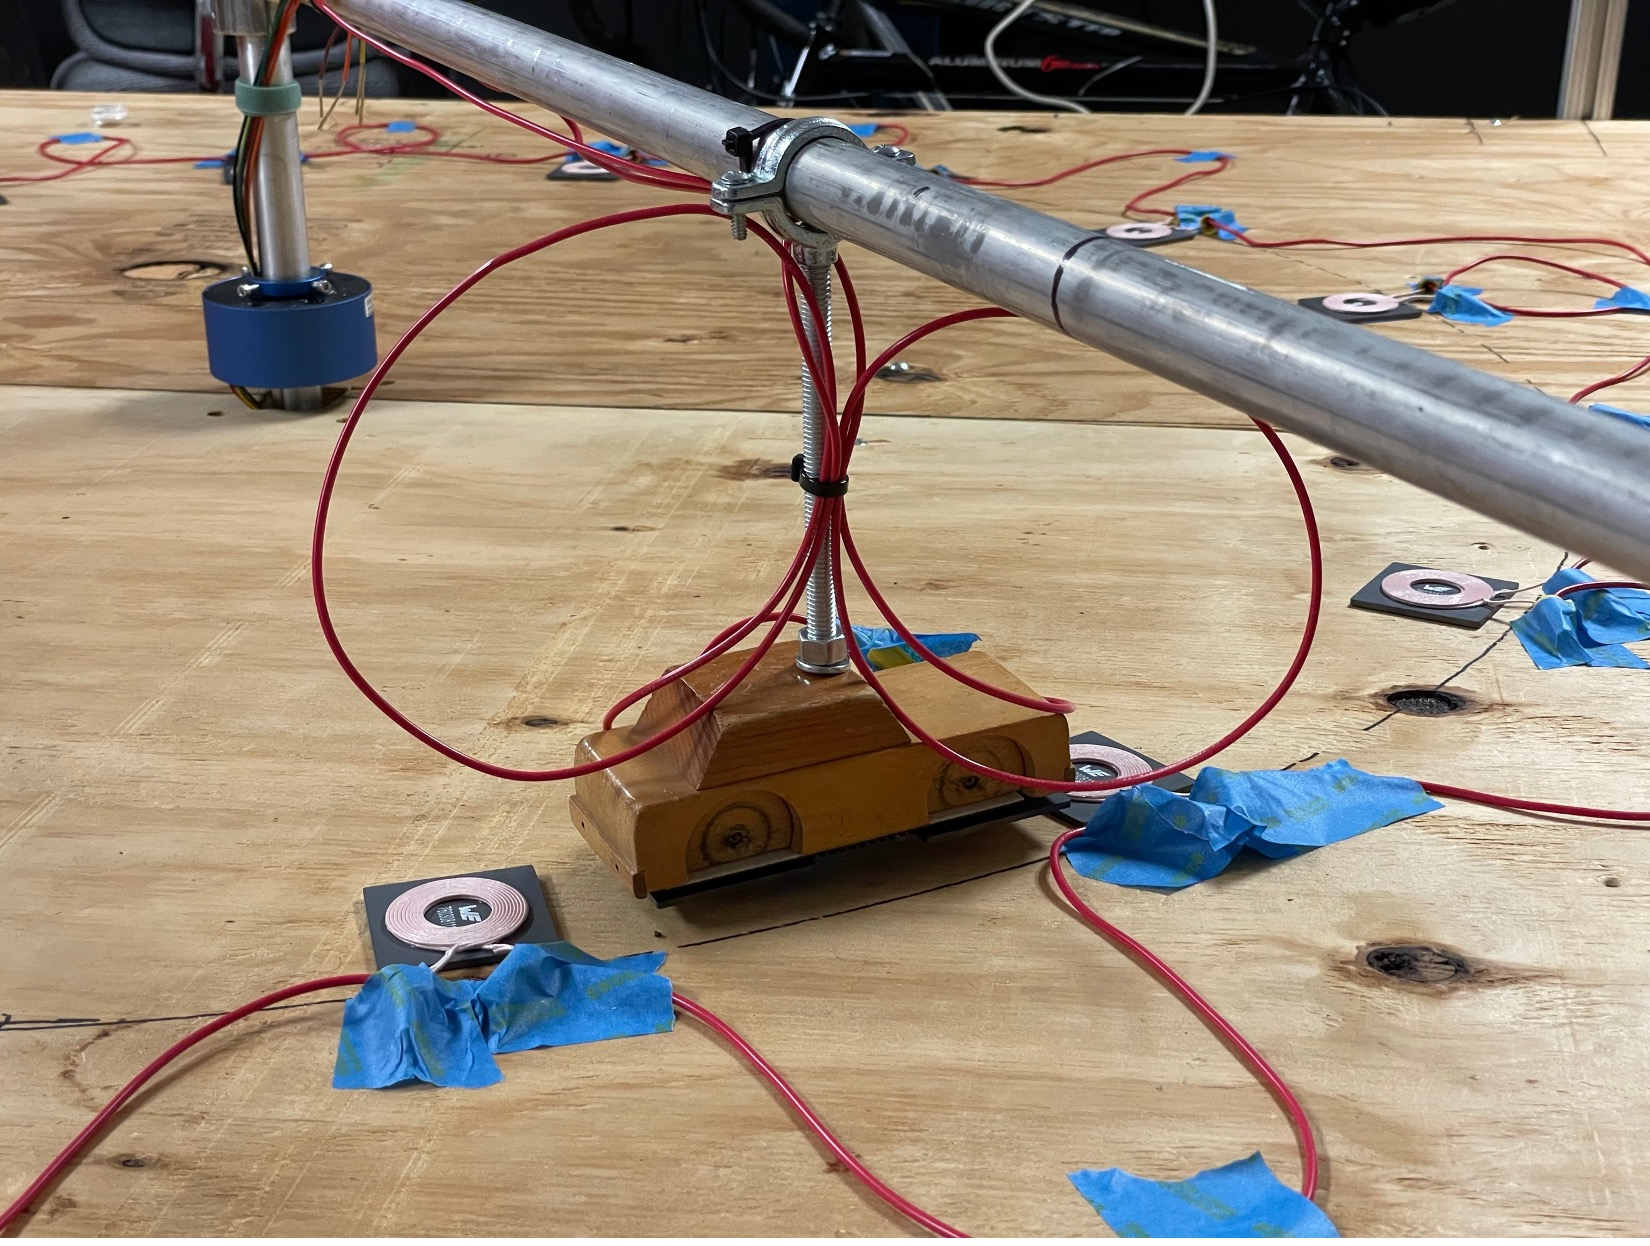
\includegraphics[width=5in]{fig8.jpg}
    \end{center}
    \renewcommand{\baselinestretch}{1}
    \small\normalsize
    \begin{quote}
    \caption[The wooden car with two transmitting coils attached]{The wooden car with two transmitting coils attached} \label{fig: f8}
    \end{quote}
\end{figure}

A wooden car is suspended from the spinning arm so that it travels over the transmitting coils. 
Two receiving coils are attached to the bottom of the wooden car to pick up the charge from the transmitting coils. 
These receiving coils are wired in series and the output is connected through the slip ring to an oscilloscope to 
gather data. The distance between the transmitting and receiving coils is less than ½ in.

\subsection{Operation of the Experimental model}
Preliminary cautions are taken into consideration prior to operation – care must be taken around voltage/current 
handling components, especially the power sources. Prior to working with the experimental model, operators must 
ensure that the deck is cleared of any obstacles or debris. A foot of distance, minimum, must be maintained 
between operators and the model while operational. When data collection is finished, operators must ensure 
that all electrical connections are detached from their respective power sources and turned off.

In order to initialize the rotational control, the power source must be connected to the motor controller. 
The frequency then has to be adjusted (from the controller) to match corresponding speeds required for data collection. 
Operators should be mindful to adjust frequencies gradually to avoid excess strain on the system. 
A tachometer is used to accurately measure the rotational speed.

For signal transmission, the output end of the transmitting coil is connected to an oscilloscope. 
Using an AC/DC signal (depending on stationary or rotational testing) via the waveform generator of the oscilloscope, 
the transmitting coil is powered. The transmitting coil is mounted to the rotating arm. 
From the oscilloscope, voltage and current are adjusted to suit the desired test data.

For recording data, a voltmeter or oscilloscope is attached to the receiving coils. 
While the experimental model is running, the induced EMF is measured and recorded on the receiving coils. 
Additionally, the relationships among the transmitting and receiving coils are recorded as well – specifically 
the turns ratio, frequency, vertical separation, and diameters.

\section{Limitations}

\subsection{Simulations}
Many assumptions made during the development will limit the applicability of the results to roads and 
decrease their accuracy, but these assumptions were necessary to make in order to construct a simulation 
that could be run in. a reasonable amount of time.

\subsubsection{Discretization}
All major computations done by the simulations are numerical in nature, meaning they are not exact since an 
exact solution is available for the multivariable integrations that are required in order to determine the 
field and flux at each point. Because the solutions are discretized, they are estimates of the actual values 
and there is more error the larger the step between each numerical calculation. Smaller steps require more 
time to calculate for the same space. Due to the large number of simulations necessary to obtain useful results, 
larger steps were used which introduced more error.  For the first and second bat h of simulations, 
the increment was set to .1 m due to time constraints, however, a preferred value is at least as small as 
.02 m because it produced < 1\% error when being used to calculate fluxes of coils in the range of our simulations. 
For our more specific recommendations, smaller steps could be used to obtain more accurate results. 
While the values may not be extremely accurate, what is important is that we have observed valuable 
trends in the data that can still help answer our research questions. 

\subsubsection{Vacuum Permeability}
In our simulations we assume vacuum permeability, as previously discussed. 
The space between the transmitting and receiving coils is not as permeable as a vacuum, 
so the flux through the receiving coil is actually smaller. Future research can incorporate 
this feature into the simulations by developing an equation for a composite material between the coils, 
but for the scope of our research this is a valid assumption because the space between the coils is mostly air.

\subsubsection{Tightness of Coils}
In the simulations we use a large value for the coils to simulate perfectly wrapped coils, but, 
coils will not be wrapped perfectly. They will likely be pancake coils. Our simulations are still applicable 
for pancake coils whose mean radius is equal to the radii used. As this is a common approximation used 
for pancake coils. Additionally, the simulation could be improved to map pancake coils instead of perfectly 
wrapped coils if desired. 

\subsubsection{Perpendicular Fields}
As previously discussed, we assume that only the z-component field contributes to the flux in the receiving coil, 
however this is not entirely accurate. Due to edge effects and small variations in the angle between the coils 
and the road surface, the coils will not be exactly parallel, so there are some effects of the x- and y-components. 
This is a reasonable assumption however, because even with small variations, the x- and y-component will 
be negligible compared to the z-component. 

\subsubsection{Uniform Fields}
A major assumption made in our simulations is that over a large distance the field variation will become uniform. 
During “start-up” and “shut-down” of the process experiences a greater change in flux, so the current at those 
locations would be greater. This is because you are transferring from a negligible field to a strong field or 
a strong field to negligible field, which is a bigger change than in the middle of the coils. 
This is a reasonable assumption based on preliminary tests run that showed that the difference is 
negligible compared to the overall change in flux.  As you can see in an example result from one of these tests 
in Figure \ref{fig: f9} to Figure \ref{fig: f12} the cumulative charge over time is very similar as well as the current over time, 
although you can see some small visible differences in the outputs. A large difference in the graphs would 
suggest that this assumption might not be valid or at least introduce significant error into our simulation, 
but it is clear that that is not the case. 

\begin{figure}
    \begin{center}
    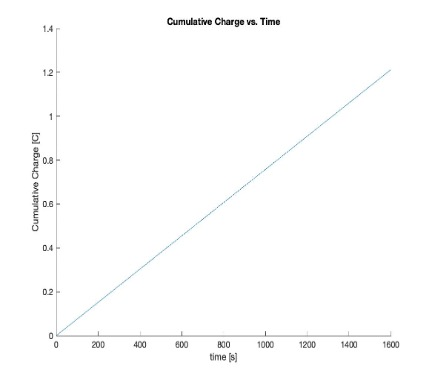
\includegraphics[width=3in]{fig9.jpg}
    \end{center}
    \renewcommand{\baselinestretch}{1}
    \small\normalsize
    \begin{quote}
    \caption[Cumulative Charge vs. Time (Not Estimated)]{Cumulative Charge vs. Time (Not Estimated)} \label{fig: f9}
    \end{quote}
\end{figure}

\begin{figure}
    \begin{center}
    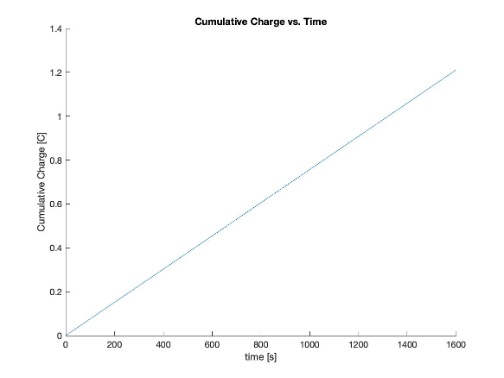
\includegraphics[width=3in]{fig10.jpg}
    \end{center}
    \renewcommand{\baselinestretch}{1}
    \small\normalsize
    \begin{quote}
    \caption[Cumulative Charge vs. Time (Estimated)]{Cumulative Charge vs. Time (Estimated)} \label{fig: f10}
    \end{quote}
\end{figure}

\begin{figure}
    \begin{center}
    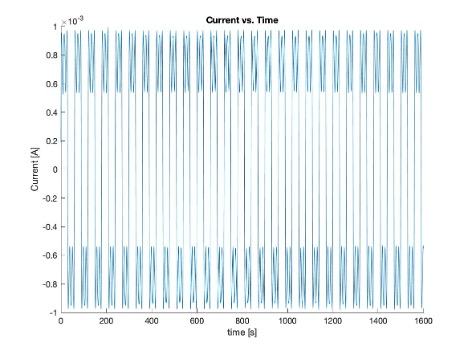
\includegraphics[width=3in]{fig11.jpg}
    \end{center}
    \renewcommand{\baselinestretch}{1}
    \small\normalsize
    \begin{quote}
    \caption[Current vs. Time (Not Estimated)]{Current vs. Time (Not Estimated)} \label{fig: f11}
    \end{quote}
\end{figure}

\begin{figure}
    \begin{center}
    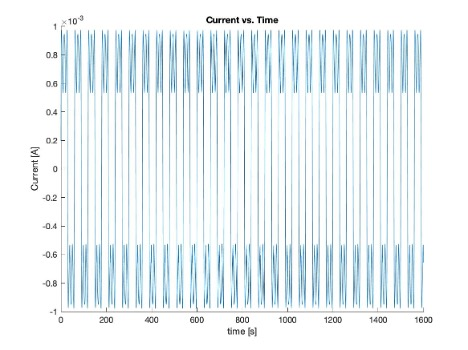
\includegraphics[width=3in]{fig12.jpg}
    \end{center}
    \renewcommand{\baselinestretch}{1}
    \small\normalsize
    \begin{quote}
    \caption[Current vs. Time (Estimated)]{Current vs. Time (Estimated)} \label{fig: f12}
    \end{quote}
\end{figure}

\subsubsection{Efficiency of the Rectifier}
In our simulations we assume that all the AC current induced in the receiving coil is converted to DC 
current without any losses. This is an overestimate, but it is a reasonable assumption because a quality 
rectifier would have negligible losses. This is also an area that can be improved on with further research.

\subsubsection{Perfect Alignment}
Our simulation assumes that the car coil can be perfectly centered above the transmitting coil at all times. 
It may be possible that drivers can remain in this position due to guides on the road and improvements in 
autonomous functions, or a mechanism like that mentioned in Section \ref{sec: s2.4.3} could be used. 
Another option would be to add a feature to the simulation to simulate poor alignment 
of the coils to determine how much of an effect misalignment has on charge output. 

\subsubsection{Constant Temperature}
Our simulation assumes a constant temperature of approximately $25^{\circ}C$. This is when the thermal 
expansion of all materials is neutral, and the resistances used in the simulation are valid. 
To address this assumption, future models will have to model resistance as function of temperature and 
consider the effects of thermal expansion and contraction of the materials in the road. 

\subsection{Experimental Model}

\subsubsection{Scalability}
The main assumption made about the applicability of the experimental model is scalability. 
The experimental model attempts to model a real-world highway on a smaller circular track. 
The alignment of the coils is not the same in a circular configuration as a highway one and 
trends observed at a smaller size might not scale very accurately to real world conditions. 
Further research will need to be done to model DWPT at more realistic highway conditions.

\subsubsection{Resources}
One other limitation we had in the construction of our experimental model was resources. 
As a Gemstone team, we had guaranteed funding of \$1800 and received an extra \$1000 from other sources. 
This limited us in terms of scope and the size of the model we could construct and test. 
Future research with more funding could build at a much bigger scale than we have. 
Additionally, an important resource we were lacking was time. This project was only ever going 
to last for four years as a Gemstone project, so we had to focus our scope again on what could 
realistically be accomplished in that timeframe. Additionally, the COVID-19 pandemic severely 
limited our amount of time in the lab with the transition to an online class structure. 
This affected our ability to gather as much data and test as many variables as we had hoped originally.

\subsubsection{Testing Variables}
There were multiple additional variables that we would have liked to have been able to test using 
our experimental model. The vertical separation between the transmitting and receiving coils was 
one of the most important ones. This was in our original plans for the model but we had to take it 
out due to the lack of time left in the project. Our original CAD model had a 3D printed part coming 
down from the arm that would have been able to be set at multiple different heights. We also wanted to 
test for the effect of an offset between the transmitting and receiving coils, where they are not perfectly 
in line with one another. Finally, one more variable we wanted to test for was the relationship between 
the sizes of the transmitting and receiving coils. To save time, we were only able to purchase one type of coil. 
This made it impossible to test for the differences between coil sizes on the receiving coil’s eventual output. 